\documentclass[tikz,border=5pt]{standalone}
\usetikzlibrary{positioning,arrows,fit}
\tikzset{%
    pics/man/.style 2 args={code={%
            % head
            \node[circle,fill,minimum size=4.5mm] (head) {};
            % body
            \node[rounded corners=2pt,minimum height=1.3cm,minimum width=0.4cm,fill,below = 1pt of head] (body) {};
            % text
            \node[below = 1pt of body] {#2};
            % arms
            \draw[line width=1mm,round cap-round cap] ([shift={(2pt,-1pt)}]body.north east) --++(-90:6mm);
            \draw[line width=1mm,round cap-round cap] ([shift={(-2pt,-1pt)}]body.north west) --++(-90:6mm);
            % legs
            \draw[ultra thick,white,-round cap] (body.south) --++(90:6.2mm);
            \node[inner ysep=0pt, fit=(head)(body)] (#1) {};
        }},
}
\definecolor{babyblue}{rgb}{0.54, 0.81, 0.94}

\begin{document}
    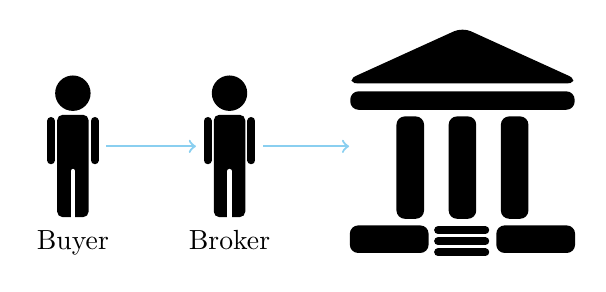
\begin{tikzpicture}

    \pic {man={buy}{Buyer}}; 
    \pic[right=50pt] {man={bro}{Broker}};   
    % stock exchange
    \node[rounded corners=3pt,minimum height=1.3cm,minimum width=0.35cm,fill, below right=-3.7em and 5em of bro] (pillar1) {};

    \node[rounded corners=3pt,minimum height=1.3cm,minimum width=0.35cm,fill,right = 8.5pt of pillar1] (pillar2) {};
    \node[rounded corners=3pt,minimum height=1.3cm,minimum width=0.35cm,fill,right = 8.5pt of pillar2] (pillar3) {};

    \node[rounded corners=3pt,minimum height=0.35cm,minimum width=1cm,fill,below left = 2pt and -12pt of pillar1] (hpillar1) {};
    \node[rounded corners=3pt,minimum height=0.35cm,minimum width=1cm,fill,below right = 2pt and -12pt of pillar3] (hpillar2) {};

    \node[rounded corners=3pt, minimum height=0.05cm, minimum width=2.85cm, fill, above = 2pt of pillar2.north] (mroof) {};

    \draw[line width=1mm, round cap-round cap] ([shift={(4.5pt,-41.3pt)}]pillar2.north east) --++(-180:7mm);
    \draw[line width=1mm, round cap-round cap] ([shift={(4.5pt,-45.3pt)}]pillar2.north east) --++(-180:7mm);
    \draw[line width=1mm, round cap-round cap] ([shift={(4.5pt,-49.3pt)}]pillar2.north east) --++(-180:7mm);

    \draw[ultra thick,fill,rounded corners=3pt] ([yshift=.7em]mroof.west) -- ([yshift=2.2em]mroof.north) -- ([yshift=.7em]mroof.east) -- cycle;
    \node[inner sep=0pt, fit=(pillar1)(mroof)(pillar3)] (SE) {};

    % arrows    
    \draw[shorten >= 2pt, shorten <= 2pt,->,thick,babyblue] (buy) -- (bro);
    \draw[shorten <= 2pt,->,thick,babyblue] (bro) -- (bro-|SE.west);

    \end{tikzpicture}

\end{document}